%%%%%%%%%%%%%%%%%%%%%%%%%%%%%%%%%%%%%%%%%
% Cheatsheet
% LaTeX Template
% Version 1.0 (12/12/15)
%
% This template has been downloaded from:
% http://www.LaTeXTemplates.com
%
% Original author:
% Michael Müller (https://github.com/cmichi/latex-template-collection) with
% extensive modifications by Vel (vel@LaTeXTemplates.com)
%
% License:
% The MIT License (see included LICENSE file)
%
%%%%%%%%%%%%%%%%%%%%%%%%%%%%%%%%%%%%%%%%%

%----------------------------------------------------------------------------------------
%	PACKAGES AND OTHER DOCUMENT CONFIGURATIONS
%----------------------------------------------------------------------------------------

\documentclass[11pt]{scrartcl} % 11pt font size

\usepackage[utf8]{inputenc} % Required for inputting international characters
\usepackage[T1]{fontenc} % Output font encoding for international characters

\usepackage[margin=0pt, landscape]{geometry} % Page margins and orientation

\usepackage{graphicx} % Required for including images

\usepackage{color} % Required for color customization
\definecolor{mygray}{gray}{.75} % Custom color

\usepackage{url} % Required for the \url command to easily display URLs
\usepackage{wrapfig}
\usepackage{tikz}

\usepackage[ % This block contains information used to annotate the PDF
colorlinks=false, 
pdftitle={Cheatsheet}, 
pdfauthor={John Smith}, 
pdfsubject={Compilation of useful shortcuts}, 
pdfkeywords={Random Software, Cheatsheet}
]{hyperref}

\setlength{\unitlength}{1mm} % Set the length that numerical units are measured in
\setlength{\parindent}{0pt} % Stop paragraph indentation

\renewcommand{\dots}{\ \dotfill{}\ } % Fills in the right amount of dots

\newcommand{\command}[2]{#1~\dotfill{}~#2\\} % Custom command for adding a shorcut

\newcommand{\sectiontitle}[1]{\paragraph{#1} \ \\} % Custom command for subsection titles

%----------------------------------------------------------------------------------------

\begin{document}

\begin{picture}(297,210) % Create a container for the page content
\tikz[remember picture,overlay] \node[opacity=0.3,inner sep=0pt] at (current page.center){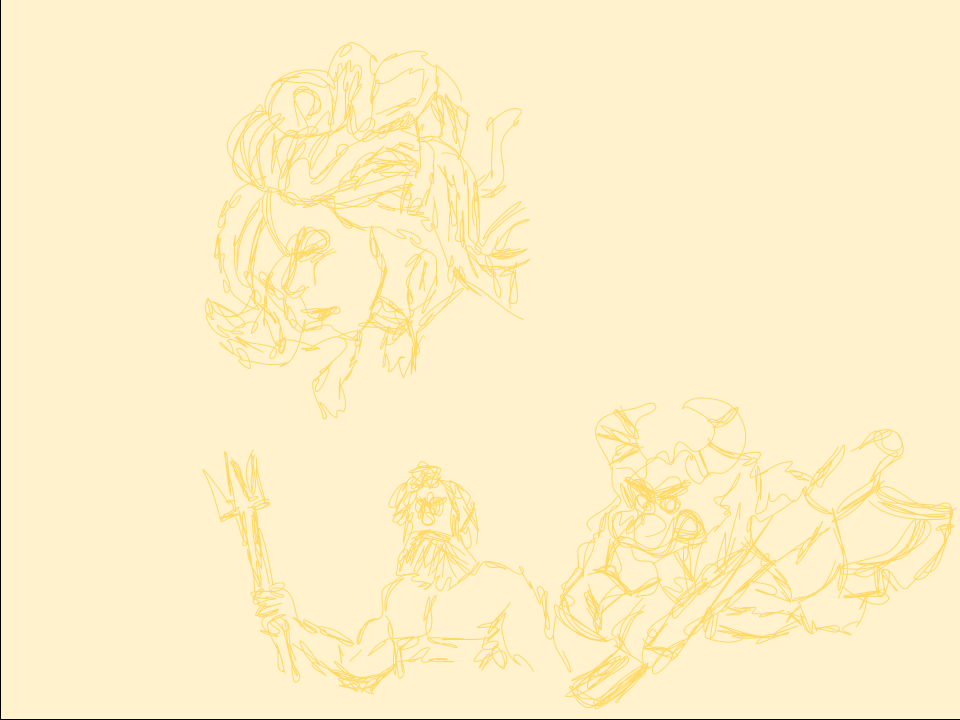
\includegraphics[width=\paperwidth,height=\paperheight]{background-img.png}};

%----------------------------------------------------------------------------------------
%	TITLE SECTION 
%----------------------------------------------------------------------------------------

\put(80,200){ % Position on the page to put the title
\begin{minipage}[t]{210mm} % The size and alignment of the title
\section*{Strife of Mythology Tower Defense - Documento de Visão} % Title
\end{minipage}
}

%----------------------------------------------------------------------------------------
%	FIRST COLUMN SPECIFICATION
%----------------------------------------------------------------------------------------

\put(10,180){ % Divide the page
\begin{minipage}[t]{85mm} % Create a box to house text

%----------------------------------------------------------------------------------------
%	HEADING ONE
%----------------------------------------------------------------------------------------

  \sectiontitle{\textit{Apresentando...}}

Strife of Mythology é um Tower Defense de tema mitológico. Suas torres evoluirão e se tornarão cada vez mais avançadas e poderosas, havendo possibilidades diferentes de torres, cada uma com suas peculiaridades. Seus inimigos, que virão diretamente da antiga mitologia (principalmente nórdica e grega), serão mais vulneráveis a certos tipos de torres, e você deverá utilizar esse fato para progredir durante o jogo.


\vspace{\baselineskip} % Whitespace before the next section
%----------------------------------------------------------------------------------------
%	HEADING TWO
%----------------------------------------------------------------------------------------				
\sectiontitle{Características}

\begin{description}
  \item [Modo \textit{endurance}] Nunca acaba! A não ser que você seja derrotado.
  \item [Torres especialistas] Certas torres são melhores contra certos tipos de inimigos.
  \item [Revenda de torres] Caso se arrependa de uma compra, é possível revender a torre.
  \item [Unico jogador] SoMTD deve ser jogado sozinho.
  \item [Sem \textit{mazing}] Os monstros fazem sempre o mesmo caminho, que não poderá ser bloqueado.
  \item [\textit{Respawn} fixo] Os monstros sempre nascem do mesmo lugar.
  \item [\textit{Vida}] O jogador começa com o valor fixo de 50 pontos de vida. Sempre que um monstro terminar o caminho predeterminado, o jogador perde uma vida e o mesmo monstro renasce do início do mapa.
  
\end{description}
%----------------------------------------------------------------------------------------

\end{minipage} % End the first column of text
} % End the first division of the page

%----------------------------------------------------------------------------------------
%	SECOND COLUMN SPECIFICATION 
%----------------------------------------------------------------------------------------

\put(105,180){ % Divide the page
\begin{minipage}[t]{85mm} % Create a box to house text

%----------------------------------------------------------------------------------------
%	HEADING FOUR
%----------------------------------------------------------------------------------------

\sectiontitle{Esquema de controle e interface}
Strife of Mythology deve ser jogado com o auxílio de um mouse e teclado. Os atalhos para acesso rápido (também chamadas de \textit{hotkeys}) facilitarão a jogabilidade, e serão possíveis com a utilização de um teclado (esses atalhos irão, por exemplo, possibilitar qual torre construir, revender uma torre rapidamente, entre outras coisas). Com o mouse, o jogador escolhe essencialmente as torres e as posições de construção.

Sobre a jogabilidade, o jogador saberá como terminar uma ação desejada através de uma interface intuitiva. Um \textit{destaque} (também chamado de \textit{highlight} e \textit{mouseover}) ocorrerá sempre que o ponteiro do mouse passar sobre uma torre. Dessa forma, o jogador poderá escolher a torre que será evoluída ou revendida passando o mouse sobre.

Sobre outros aspectos da interface, o jogo ainda contará com um menu com diversas opções, possibilitando mudanças no volume do áudio do jogo, e visualização de uma lista com todos os comandos e atalhos disponíveis.

%----------------------------------------------------------------------------------------
%	HEADING FIVE
%----------------------------------------------------------------------------------------				
					
% \sectiontitle{Descrição Tecnológica} % Heading five
\vspace{\baselineskip} % Whitespace before the next section
%----------------------------------------------------------------------------------------

\end{minipage} % End the second column of text
} % End the second division of the page

%----------------------------------------------------------------------------------------
%	THIRD COLUMN SPECIFICATION 
%----------------------------------------------------------------------------------------

\put(200,180){ % Divide the page
\begin{minipage}[t]{85mm} % Create a box to house tex



%----------------------------------------------------------------------------------------
%	HEADING THREE
%----------------------------------------------------------------------------------------	

\sectiontitle{Público e Plataforma Alvo}
O jogo tem como principal alvo os entusiastas de \textit{tower defenses} e de jogos de tema mitológico. Por conta das características da arte do jogo, o SoMTD não é muito recomendado para crianças, mas sim para um público mais maduro. Além disso, por conta do fator desafio, o jogo provavelmente atrairá a atenção de \textit{gamers} em geral.


\vspace{\baselineskip} % Whitespace before the next section

%----------------------------------------------------------------------------------------
%	IMPORTANT FILES
%----------------------------------------------------------------------------------------

% \sectiontitle{Relação dos Logotipos}
%
% \begin{figure}
%   \begin{center}
%     \includegraphics[scale=0.2]{Sdl-logo.png}
%   \end{center}
%   % \caption{SDL é uma das bibliotecas que possibilitarão o jogo em si. Ela fornece uma maneira de comunicar diretamente com recursos do computador, além de oferecer outras funcionalidades.}
% \end{figure}
%
% \includegraphics[scale=0.2]{neovim-logo.png}

% \vspace{\baselineskip} % Whitespace before the next section
% \vspace{\baselineskip} % Whitespace before the next section

\sectiontitle{Equipe}
Você pode nos encontrar na UnB - Campus Gama. Sugestões e novas funcionalidades devem ser sugeridas via \textit{issues} em \href{https://github.com/StrifeOfMythologyTD/SoMTD/issues}{nosso repositório}. Nosso e-mail para contato é: \href{mailto:strifeofmythology@gmail.com}{strifeofmythology@gmail.com}

\end{minipage} % End the third column of text
} % End the third division of the page
\end{picture} % End the container for the entire page

%----------------------------------------------------------------------------------------

\end{document}
